\documentclass{article}
\usepackage[margin=1in]{geometry}
\usepackage{amsmath,amsthm,amssymb}
\usepackage{bbm,enumerate,mathtools}
\usepackage{tikz,pgfplots}
\usepackage{chessboard}
\usepackage[hidelinks]{hyperref}
\usepackage{multicol} % Problem 35
\usepackage{xstring} % Difficulty command
\usetikzlibrary{shapes.geometric}

\newenvironment{question}{\begin{trivlist}\item[\textbf{Question.}]}{\end{trivlist}}
\newenvironment{note}{\begin{trivlist}\item[\textbf{Note.}]}{\end{trivlist}}
\newenvironment{references}{\begin{trivlist}\item[\textbf{References.}]}{\end{trivlist}}
\newenvironment{related}{\begin{trivlist}\item[\textbf{Related.}]\end{trivlist}\begin{enumerate}}{\end{enumerate}}

\newcommand\score[1]{
\pgfmathsetmacro\pgfxa{#1+1}
\tikzstyle{scorestars}=[
  star,
  star points=5,
  star point ratio=2.25,
  draw,
  inner sep=3pt,
  anchor=outer point 5
]
  \begin{tikzpicture}[baseline]
    \draw[opacity=0] (0,-0.5) rectangle (0,0.2); % Workaround for whitespace at the bottom.
    \foreach \i in {1,...,4} {
      \pgfmathparse{(\i<=#1?"yellow":"gray")}
      \edef\starcolor{\pgfmathresult}
      \draw (\i*4.5ex,0) node[name=star\i,scorestars,fill=\starcolor]  {};
    }
  \end{tikzpicture}
}

\newcommand{\difficulty}[1]{%
  \IfEqCase{#1}{%
      {1}{
        
\begin{tikzpicture}[scale=0.7, baseline=0.9mm]%
          \definecolor{slopegreen}{rgb}{0.0, 0.5, 0.0}%
          \fill[slopegreen] (0.5,0.5) circle (0.5);%
        \end{tikzpicture}%
      }%
      {2}{
        
\begin{tikzpicture}[scale=0.7, baseline=0.9mm]%
          \definecolor{slopeblue}{rgb}{0.0, 0.44, 1.00}
          \fill[slopeblue] (0,0) rectangle (1,1);%
        \end{tikzpicture}%
      }%
      {3}{
\begin{tikzpicture}[scale=0.7, baseline=0.9mm]\fill (0,0.5)--(0.5, 0)--(1,0.5)--(0.5,1)--cycle; \end{tikzpicture}}%
      {4}{
\begin{tikzpicture}[scale=0.7, baseline=0.9mm]\fill (0.25,0)--(0,0.5)--(0.25,1)--(0.5,0.5)--cycle; \fill (0.75,0)--(0.5,0.5)--(0.75,1)--(1,0.5)--cycle;\end{tikzpicture}}%
      % you can add more cases here as desired
  }[\PackageError{difficulty}{Undefined difficulty level: #1}{}]%
}%
\newcommand{\rating}[2]{\difficulty{#1}\\\score{#2}\\}


\begin{document}
\rating{3}{3}
Let $G$ be some $n \times m$ grid as in Figure 1, where each cell has two
opposite diagonals connected (uniformly at random).
Choose a cell (also uniformly at random), and consider the component that goes through this cell.
\begin{figure}[!h]
  \centering
  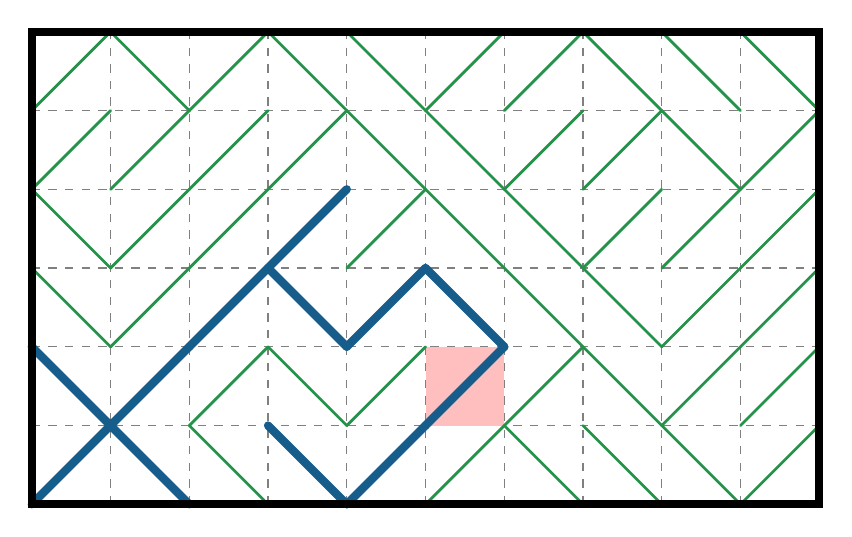
\begin{tikzpicture}[scale=1]
    \draw[gray, dashed] (0,0) grid (10,6);
    \fill[red!25] (5,1) rectangle (6,2);
    \foreach \a/\b/\s/\t in {
      0/5/1/1, 1/5/0/1, 2/5/1/1, 3/5/0/1, 4/5/0/1, 5/5/1/1, 6/5/1/1, 7/5/0/1, 8/5/0/1, 9/5/0/1,
      0/4/1/1, 1/4/1/1, 2/4/1/1, 3/4/1/1, 4/4/0/1, 5/4/0/1, 6/4/1/1, 7/4/1/1, 8/4/0/1, 9/4/1/1,
      0/3/0/1, 1/3/1/1, 2/3/1/1, 3/3/1/3, 4/3/1/1, 5/3/0/1, 6/3/0/1, 7/3/1/1, 8/3/1/1, 9/3/1/1,
      0/2/0/1, 1/2/1/1, 2/2/1/3, 3/2/0/3, 4/2/1/3, 5/2/0/3, 6/2/0/1, 7/2/0/1, 8/2/1/1, 9/2/1/1,
      0/1/0/3, 1/1/1/3, 2/1/1/1, 3/1/0/1, 4/1/1/1, 5/1/1/3, 6/1/1/1, 7/1/0/1, 8/1/1/1, 9/1/1/1,
      0/0/1/3, 1/0/0/3, 2/0/0/1, 3/0/0/3, 4/0/1/3, 5/0/1/1, 6/0/0/1, 7/0/0/1, 8/0/0/1, 9/0/1/1
    } {
      \draw[line cap=round, line width=\t, draw={rgb:red,0.5;green,2;blue,\t}]
        (\a, \b + 1 - \s)--(\a + 1, \b + \s )
      ;
    }
    \draw[line width=3] (0,0) rectangle (10,6);
  \end{tikzpicture}
  \caption{
    An example of a $6 \times 10$ grid, where a component of size $12$ has been selected.
  }
\end{figure}

\begin{question}
  What is the expected size of the selected component?
\end{question}

\begin{related}
  \item What is the expected number of components in an $n \times m$ grid?
  \item How long is the longest component expected to be?
  \item How does this change if the grid on a torus/cylinder/M\"obius strip/etc?
\end{related}
\end{document}
